\phantomsection
\addcontentsline{toc}{chapter}{Appendices}

\section{Appendices A ( Screenshots )}

\begin{figure}[htb]
    \centering
    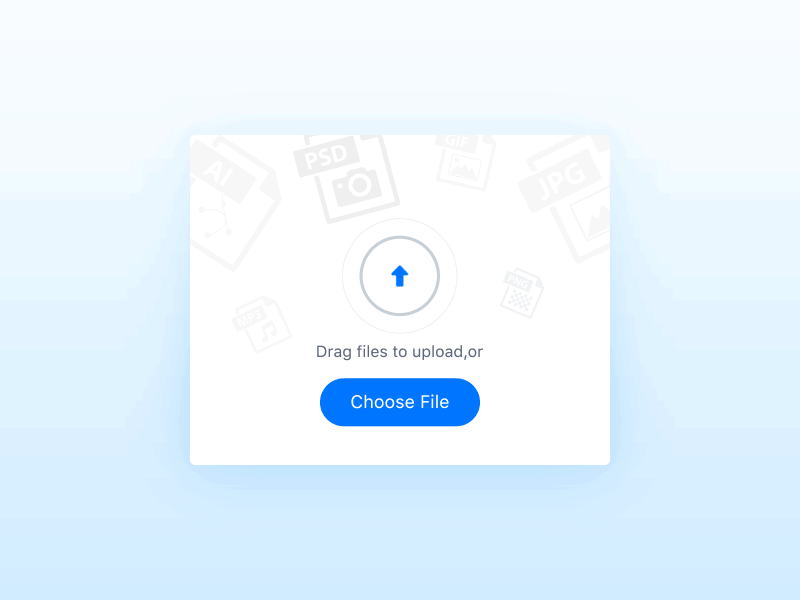
\includegraphics[width=\textwidth]{up.png}
    \caption{Upload screen}
    \label{fig:modeldd}
\end{figure}

\begin{figure}[htb]
    \centering
    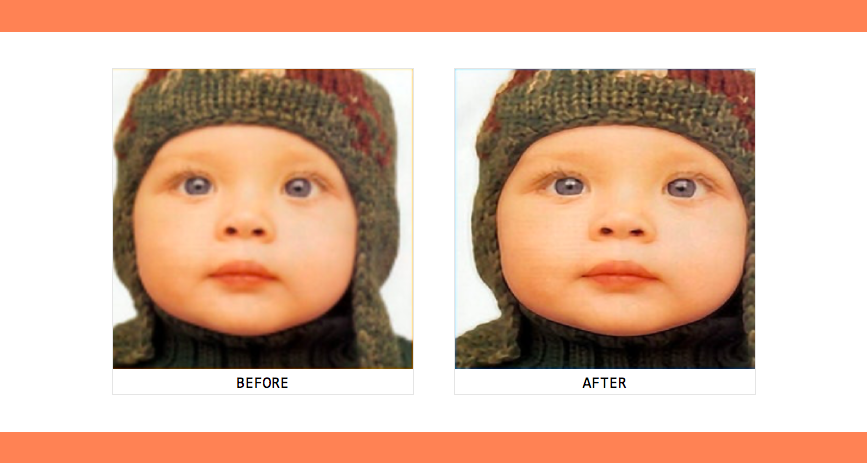
\includegraphics[width=\textwidth]{shot.png}
    \caption{Image result screen}
    \label{fig:modeldd}
\end{figure}

\section{Appendices B ( Source Code )}

\subsection{Python Flask POST}

\lstinputlisting[language=python]{code/flask.py}

\subsection{React component}

\lstinputlisting[language=javascript]{code/react.js}

\subsection{Keras model}

\lstinputlisting[language=python]{code/model.py}